%% Creator: Inkscape inkscape 0.48.0, www.inkscape.org
%% PDF/EPS/PS + LaTeX output extension by Johan Engelen, 2010
%% Accompanies image file 'h_separation_base.ps' (pdf, eps, ps)
%%
%% To include the image in your LaTeX document, write
%%   \input{<filename>.pdf_tex}
%%  instead of
%%   \includegraphics{<filename>.pdf}
%% To scale the image, write
%%   \def\svgwidth{<desired width>}
%%   \input{<filename>.pdf_tex}
%%  instead of
%%   \includegraphics[width=<desired width>]{<filename>.pdf}
%%
%% Images with a different path to the parent latex file can
%% be accessed with the `import' package (which may need to be
%% installed) using
%%   \usepackage{import}
%% in the preamble, and then including the image with
%%   \import{<path to file>}{<filename>.pdf_tex}
%% Alternatively, one can specify
%%   \graphicspath{{<path to file>/}}
%% 
%% For more information, please see info/svg-inkscape on CTAN:
%%   http://tug.ctan.org/tex-archive/info/svg-inkscape

\begingroup
  \makeatletter
  \providecommand\color[2][]{%
    \errmessage{(Inkscape) Color is used for the text in Inkscape, but the package 'color.sty' is not loaded}
    \renewcommand\color[2][]{}%
  }
  \providecommand\transparent[1]{%
    \errmessage{(Inkscape) Transparency is used (non-zero) for the text in Inkscape, but the package 'transparent.sty' is not loaded}
    \renewcommand\transparent[1]{}%
  }
  \providecommand\rotatebox[2]{#2}
  \ifx\svgwidth\undefined
    \setlength{\unitlength}{333.748pt}
  \else
    \setlength{\unitlength}{\svgwidth}
  \fi
  \global\let\svgwidth\undefined
  \makeatother
  \begin{picture}(1,0.35316167)%
    \put(0,0){\includegraphics[width=\unitlength]{pics/h_separation_base.ps}}%
    \put(0.18629325,0.03){\makebox(0,0)[lb]{\smash{$200$}}}%
    \put(0.268487,0.03){\makebox(0,0)[lb]{\smash{$400$}}}%
    \put(0.35124705,0.03){\makebox(0,0)[lb]{\smash{$600$}}}%
    \put(0.43372245,0.03){\makebox(0,0)[lb]{\smash{$800$}}}%
    \put(0.5090817,0.03){\makebox(0,0)[lb]{\smash{$1000$}}}%
    \put(0.59158407,0.03){\makebox(0,0)[lb]{\smash{$1200$}}}%
    \put(0.67408344,0.03){\makebox(0,0)[lb]{\smash{$1400$}}}%
    \put(0.75658281,0.03){\makebox(0,0)[lb]{\smash{$1600$}}}%
    \put(0.83908218,0.03){\makebox(0,0)[lb]{\smash{$1800$}}}%
    \put(0.50063221,-0.02){\makebox(0,0)[lb]{\smash{$f$\,(кГц)}}}%
    \put(0.05,0.0619){\makebox(0,0)[lb]{\smash{$-40$}}}%
    \put(0.05,0.12811762){\makebox(0,0)[lb]{\smash{$-30$}}}%
    \put(0.05,0.19433525){\makebox(0,0)[lb]{\smash{$-20$}}}%
    \put(0.05,0.26055287){\makebox(0,0)[lb]{\smash{$-10$}}}%
    \put(0.094,0.32677349){\makebox(0,0)[lb]{\smash{$0$}}}%
    \put(0.02,0.16467814){\rotatebox{90}{\makebox(0,0)[lb]{\smash{$A$\,(дБ)}}}}%
    %\put(0.76810348,0.28268933){\makebox(0,0)[lb]{\smash{$r$=0cm}}}%
  \end{picture}%
\endgroup
